%--------------------------------------
% Create title frame
\titleframe

%--------------------------------------
% Table of contents
\begin{frame}{Overview}
  \setbeamertemplate{section in toc}[sections numbered]
  \tableofcontents[hideallsubsections]
\end{frame}

\section{Introduction}

% What will we learn slide
\begin{frame}{What will we learn today?}
    \small
    \begin{itemize}
        \item The transmission line
        \item An introduction to power flow analysis
    \end{itemize}
    You will be able to do exercises 4.3, 4.4, 4.6, 4.7, 4.8, 4.9, 4.10, 4.11, 4.12, Lab4 (power-flow in python), 5.1, 5.2, 5.5, 5.6 from the Ned Mohan's book.
\end{frame}

% Video slide
\begin{frame}
    \begin{figure}
        \centering
        \href{https://www.youtube.com/embed/R_Z-A9KZr58}{\underline{Introduction video link}}
    \end{figure}
\end{frame}

% Definition
\begin{frame}{Definition}
    \begin{itemize}
        \item An (overhead) transmission line is a set of 3 bundles of conductors corresponding to the three phases of the system.
        \item Commonly used voltages range from 70 kV to 380 kV in Belgium (more where distances are larger).
        \item Minimum distances between conductors depend on the voltage level, and thus electrical properties also depend on the voltage level.
        \item Underground cables are more and more used. They can be modeled in a similar way as overhead transmission lines, but hey have different properties.
    \end{itemize}
\end{frame}

% ELIA's network
\begin{frame}{A part of ELIA's network}
    \centering
    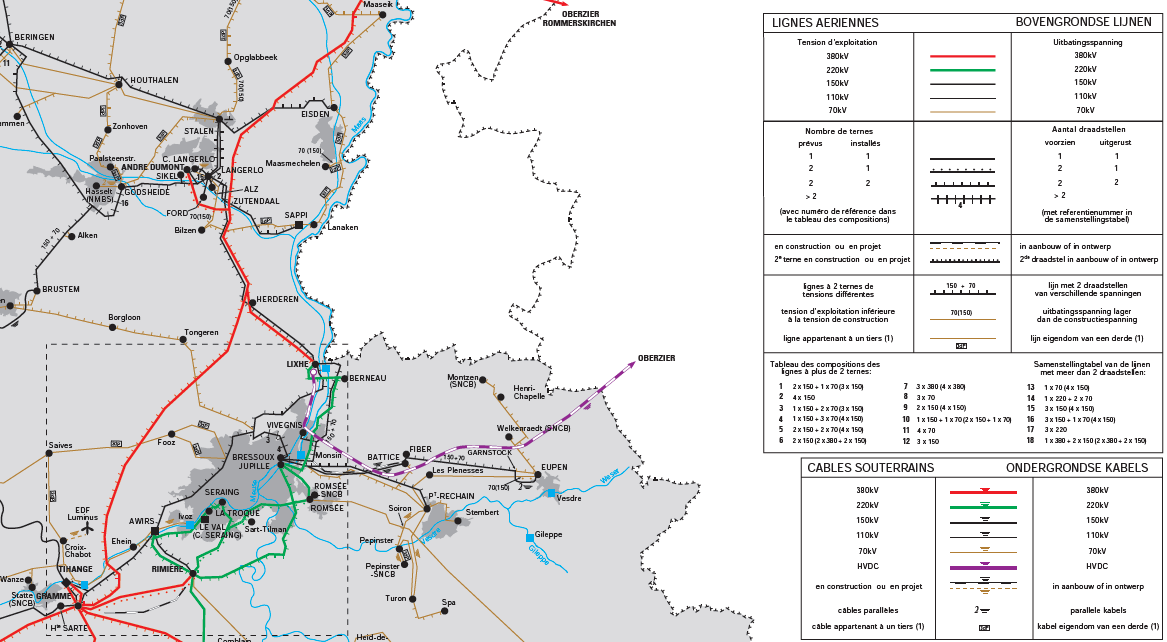
\includegraphics[width=0.7\textwidth]{images/carte_ELIA_2019_Liege.png}\\
    Source: \href{https://www.elia.be/fr/infrastructure-et-projets/nos-infrastructures}{https://www.elia.be/fr/infrastructure-et-projets/nos-infrastructures}
\end{frame}

% Transmission line parameters
\begin{frame}{Transmission line parameters}
\begin{columns}
    \begin{column}{0.5\textwidth}
    A \textit{chunk} (a tiny piece)  of transmission line can be represented as:
    \begin{center}
        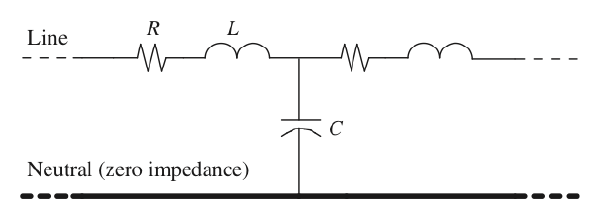
\includegraphics[width=\textwidth]{images/TL_1.png}
    \end{center}
    with $R$, $L$ and $C$ expressed \textbf{per unit of length}.
    \end{column}
    \begin{column}{0.5\textwidth}
    where
    \begin{itemize}
        \item $R$ represents the series resistance, as small as possible to minimize $RI^2$ (influence of the frequency and skin effect)
        \item the series inductance $L$ models the magnetic coupling between phases
        \item the shunt capacitance $C$ models the capacitive coupling between phases
        \item a shunt conductance $G$ can be added to model e.g. the leakage current through insulators
    \end{itemize}
    \end{column}
\end{columns}
\end{frame}

\begin{frame}{Typical cross section of a high voltage overhead conductor}
    
\begin{columns}

    \begin{column}{0.56\textwidth}
        Skin depth (detph at which decay of current density is $1/e$ of surface density):\\[\baselineskip]
        \begin{tabular}{l r r}
        Material & Frequency [Hz] & depth [mm]\\
        \hline
        Copper & 50 & 9.4 \\
        Copper & 60 & 8.6 \\
        Aluminum & 50 & 12.0 \\
        Aluminum & 60 & 10.9\\
    \end{tabular}
    \end{column}
    \begin{column}{0.4\textwidth}
        \centering
        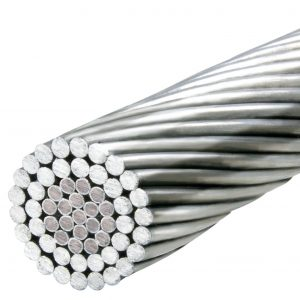
\includegraphics[width=0.8\textwidth]{images/conductor-300x300.jpg}
    \end{column}
    
\end{columns}




\end{frame}

\begin{frame}{Approximate Overhead Transmission Line Parameters}
For bundled conductors at 60 Hz.

\begin{columns}
    \begin{column}{0.55\textwidth}
\begin{table}
\begin{tabular}{rrrr}
\hline Nominal  & $\boldsymbol{R}$ & $\omega L$& $\omega \boldsymbol{C}$ \\
Voltage & $(\boldsymbol{\Omega} / \mathbf{k m})$ & $(\boldsymbol{\Omega} / \mathbf{k m})$ & $ (\boldsymbol{\mu} \boldsymbol{\mho} / \mathbf{k m})$ \\
\hline 230 kV & 0.06 & 0.50 & 3.4 \\
345 kV & 0.04 & 0.38 & 4.6 \\
500 kV & 0.03 & 0.33 & 5.3 \\
765 kV & 0.01 & 0.34 & 5.0 \\
\hline
\end{tabular}
\end{table}
    \end{column}
    \begin{column}{0.4\textwidth}
    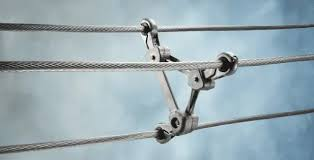
\includegraphics[width=\textwidth]{images/bundled_conductors.jpeg}
    \end{column}
\end{columns}
\end{frame}

\begin{frame}{Approximate underground cable parameters}
For conductors at 60 Hz.
\begin{columns}
    \begin{column}{0.55\textwidth}
\begin{table}
\begin{tabular}{rrrr}
\hline Nominal  & $\boldsymbol{R}$ & $\omega L$& $\omega \boldsymbol{C}$ \\
Voltage & $(\boldsymbol{\Omega} / \mathbf{k m})$ & $(\boldsymbol{\Omega} / \mathbf{k m})$ & $ (\boldsymbol{\mu} \boldsymbol{\mho} / \mathbf{k m})$ \\
\hline 
110 kV	& 0.05	& 0.030	&  95 \\
220 kV	& 0.04	& 0.025	& 115\\
330 kV	& 0.03	& 0.020	& 130\\
400 kV	& 0.02	& 0.018	& 150\\
\hline
\end{tabular}
\end{table}
    \end{column}
    \begin{column}{0.4\textwidth}
    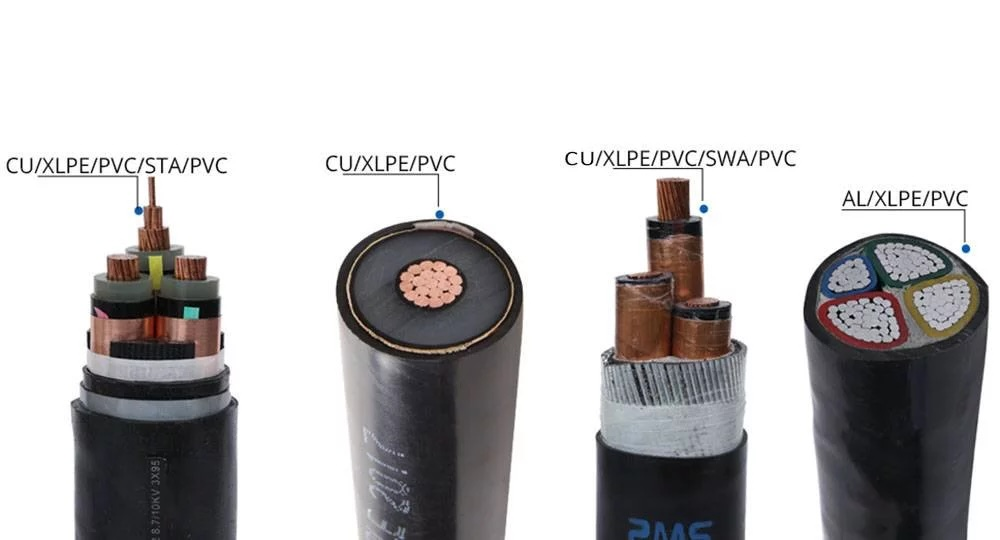
\includegraphics[width=\textwidth]{images/Cable-Electrico-Subterraneo.jpeg}
    \end{column}
\end{columns}
\end{frame}

\section{Distributed model}
% Distributed parameter representation
\begin{frame}[allowframebreaks]{Distributed parameter representation}
    We consider that we are in sinusoidal steady state. 
    On a per-phase basis, the line can be represented as many chunks connected to each other:  
    \begin{center}
        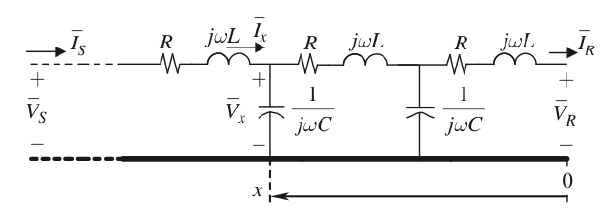
\includegraphics[width=0.75\textwidth]{images/TL_distributed.png}
    \end{center}
    \textbf{How do voltage and current evolve as a function of the position on the line?}

    \begin{itemize}
        \item As $R$ is small, let's assume $R$ is considered as \textit{lumped} (a discrete resistive element on one side of the line)
        \item $\frac{d\bar{V}(x)}{dx} = j\omega L \bar{I}(x)$
        \item $\frac{d\bar{I}(x)}{dx} = j\omega C \bar{V}(x)$
    \end{itemize}

    Hence $$\frac{d^2\bar{V}(x)}{dx^2} + \beta^2 \bar{V}(x) = 0$$
    with $\beta = \omega \sqrt{LC}$ the \textit{propagation constant}
\end{frame}
\begin{frame}[allowframebreaks]{Solution of the ODE}

    The previous equation has a solution of the type 
    $$\bar{V}(x) = \bar{V}_1 e^{\beta j x} + \bar{V}_2 e^{-\beta j x}.$$
    
        
    By derivation, the current is  $$\bar{I}(x) = (\bar{V}_1 e^{\beta j x} - \bar{V}_2 e^{-\beta j x}) / Z_c.$$
    
    With the \textbf{surge impedance} $$Z_c = \sqrt{\frac{L}{C}}.$$
    
    The boundary conditions at $x=0$, $$\bar{V}(0) = \bar{V}_R = V_R \angle 0,$$  and $$\bar{I}(0) = \bar{I}_R$$
    allow to determine constants $\bar{V}_1$ and $\bar{V}_2$, and finally
    $$
    \bar{V}(x) = \bar{V}_R \cos(\beta x) + j Z_c \bar{I}_R \sin(\beta x).
    $$
\end{frame}

\section{Surge impedance loading}
\begin{frame}{Closing the line on the surge impedance $Z_c$}
    If the line is assumed lossless and \textit{we close it with $Z_c$}, assuming $\bar{V}_R = V_R \angle 0$:
    \begin{center}
        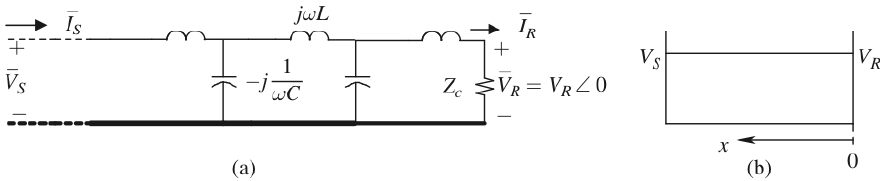
\includegraphics[width=\textwidth]{images/SIL.png}
    \end{center}
    then the voltage \textit{magnitude is constant} over the line: $\bar{V}(x) = V_R e^{j\beta x}$, and only the \textit{angle increases with $x$}.
    Similar conclusion for $\bar{I}(x)$.
    \begin{itemize}
        \item Why? The reactive power consumed by the line is the same as the reactive power produced, everywhere.
    \end{itemize}
\end{frame}

% Illustration in Python
\begin{frame}{Illustration in Python}
\begin{columns}
    \begin{column}{0.55\textwidth}
    \begin{center}
        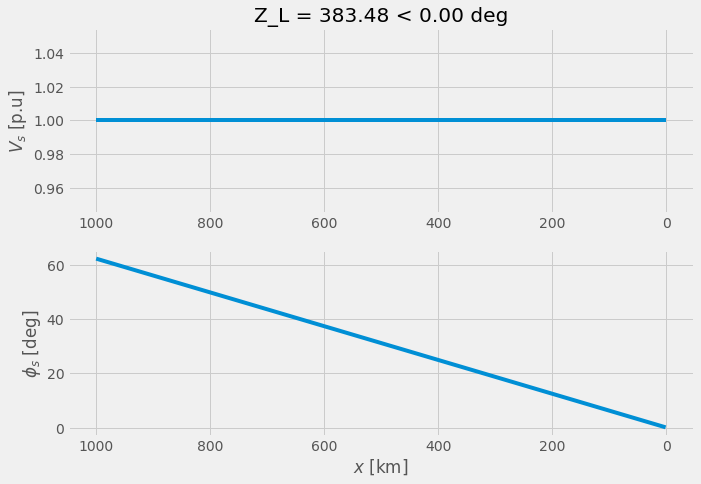
\includegraphics[width=\textwidth]{images/line_model_voltage.png}
        \small{SIL, 230 kV line params}
    \end{center}
    \end{column}
    \begin{column}{0.4\textwidth}
    See the \href{https://colab.research.google.com/drive/1FDHjHhW1a6JECWwfznBeP2T5-M9UaJn8?usp=sharing}{\underline{Python notebook}}.
    \end{column}
\end{columns}

\end{frame}

% Zc and SIL
\begin{frame}{Surge impedance loading}
    $Z_c$ depends on the line characteristics/geometry and is, hence, mainly a function of the voltage level (distances between conductors, etc.).

    The surge impedance loading (SIL) is the power drawn by the load $Z_c$, which depends on the voltage level $V_{LL}$
    $$
    SIL = \frac{V^2_{LL}}{Z_c}
    $$


    Example: for $500 \text{ kV}$, $SIL \approx 1020 \text{ MW}.$
\end{frame}

% Line loadability
\begin{frame}{Line loadability}
    The SIL gives an idea of the loadability of a line depending on its length:
    \begin{itemize}
        \item short line, $ l < 100 \text{ km}$
        \begin{itemize}
            \item load limit $= 3 \times SIL$
            \item thermal limit (See Section~\ref{sec:LR} on Line rating)
        \end{itemize}
        \item Medium length line, $ 100 \text{ km} < l < 300 \text{ km}$
        \begin{itemize}
            \item load limit $= 1.5$ to $3 \times SIL$
            \item voltage drop $< 5\%$
        \end{itemize}
        \item Long line, $ l > 300 \text{ km}$
        \begin{itemize}
            \item load limit $\approx 1 \times SIL$
            \item for system stability, the angle difference between line ends should stay $< 40^\circ$, see lecture on Transient stability.
        \end{itemize}
    \end{itemize}
\end{frame}


\section{Lumped transmission line model}
\begin{frame}{The $\pi$ model}
If $l$ is relatively small ($< 300 \text{ km}$), we can \textit{approximate} the line with \textbf{lumped} parameters,
\begin{columns}
    \begin{column}{0.55\textwidth}
    \begin{center}
        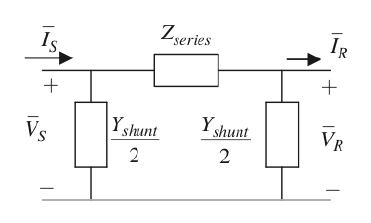
\includegraphics[width=\textwidth]{images/pi_1.png}
    \end{center}
    \end{column}
    \begin{column}{0.45\textwidth}
    with, by manipulation of the previous equations and assuming $\beta l$ small,
    \begin{itemize}
        \item $Z_{\text{series}} = R l +  j \omega L l$
        \item $\frac{Y_{\text{shunt}}}{2} = j \frac{\omega C l}{2}$
    \end{itemize}
    
    Remember that $R$, $L$ and $C$ are per km values.

    This $\pi$ model is symmetrical by design.
    \end{column}
\end{columns}

    
\end{frame}

% Illustration in Python
\begin{frame}{Illustration in Python}

\begin{columns}
    \begin{column}{0.55\textwidth}
    \begin{center}
        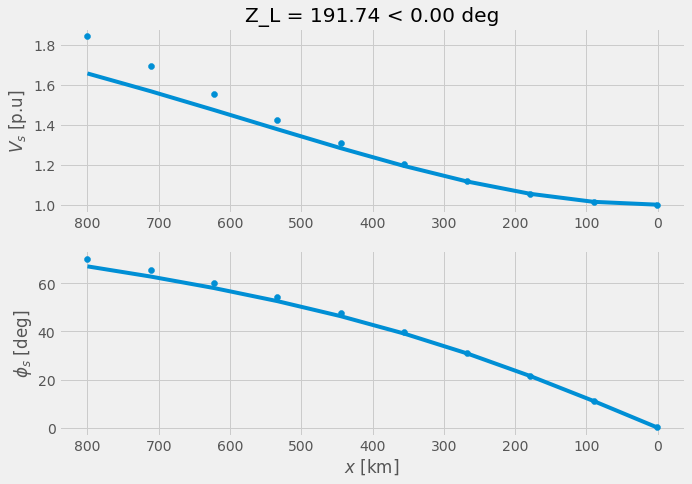
\includegraphics[width=\textwidth]{images/pi_model_voltage.png}
        \small{SIL, 230 kV line params}
    \end{center}
    \end{column}
    \begin{column}{0.4\textwidth}
    Dots are obtained with the $\pi$ model, while plain lines are from the distributed model. The approximation error grows for $l > 300$ km.

    See this \href{https://colab.research.google.com/drive/1FDHjHhW1a6JECWwfznBeP2T5-M9UaJn8?usp=sharing}{\underline{Python notebook}}.
    \end{column}
\end{columns}
\end{frame}

\section{Line rating}\label{sec:LR}
\begin{frame}[allowframebreaks]{Static line rating}

The \textbf{Static Line Rating} is the maximum continuous current a transmission line can carry under a specific set of predefined, fixed environmental conditions.

This rating is primarily constrained by \textbf{thermal limits} to ensure the safe and reliable operation of the line.

\begin{itemize}
\item \textbf{Conductor Thermal Limit:}
\begin{itemize}
\item The conductor's electrical resistance generates heat ($RI^2$).
\item This heat must be balanced by cooling from the environment.
\item An excessive temperature can cause:
\begin{enumerate}
\item \textbf{Increased Sag:} Conductor expansion due to heat causes the line to sag, potentially violating minimum clearance requirements to the ground, buildings, or other infrastructure.
\item \textbf{Material Damage:} Prolonged high temperatures can anneal the conductor, reducing its tensile strength and lifespan.
\end{enumerate}
\end{itemize}

\item \textbf{Environmental Conditions:}
\begin{itemize}
    \item The "static" nature of the rating comes from assuming a fixed set of weather parameters.
    \item \textbf{Ambient Air Temperature:} A baseline temperature (e.g., $40^{\circ}C$) is used. Higher temperatures reduce the cooling capability of the air.
    \item \textbf{Wind Speed:} A low, static wind speed (e.g., $2 \text{ ft/s}$ at a $45^{\circ}$ angle) is assumed to provide minimal convective cooling. Higher wind speeds would allow for more current.
    \item \textbf{Solar Radiation:} A fixed value for solar heat gain is included, assuming a specific level of direct sunlight on the conductor.
\end{itemize}

\end{itemize}

Static line ratings are a conservative and fundamental safety measure. They represent the worst-case continuous scenario to prevent physical damage and clearance violations under predictable conditions.


\end{frame}
% Video slide
\begin{frame}{Dynamic line rating}
    \begin{figure}
        \centering
        \href{https://www.youtube.com/embed/pzYvDuvM5JY}{{\underline{Dynamic line rating video link}}}
    \end{figure}
\end{frame}
